\documentclass[a4paper,10pt]{report}

%%%% PRATIQUE POUR LES ALINEAS CHIANTS
\usepackage{indentfirst}

\usepackage[colorlinks=false]{hyperref}

%%%% POUR L'OPTION LABEL= %%%
\usepackage{enumitem}

\setlength{\parindent}{30pt}
\setlength{\parskip}{1ex}
\setlength{\textwidth}{15cm}
\setlength{\textheight}{24cm}
\setlength{\oddsidemargin}{0.2cm}
\setlength{\evensidemargin}{-.7cm}
\setlength{\topmargin}{-.5in}

\usepackage{graphicx}
\usepackage{titling}
\usepackage{listings}
\lstset{%
  basicstyle=\scriptsize\sffamily,%
  commentstyle=\footnotesize\ttfamily,%
  frameround=trBL,
  frame=single,
  breaklines=true,
  showstringspaces=false,
  numbers=left,
  numberstyle=\tiny,
  numbersep=10pt,
  keywordstyle=\bf
}
\newcommand{\subtitle}[1]{%
  \posttitle{%
    \par\end{center}
    \begin{center}\large#1\end{center}
    \vskip0.5em}%
}

%%%%%%%%%%%%%%%% PAGE DE GARDE %%%%%%%%%%%%%%%%%%%%%%
% Crédit : http://www.grappa.univ-lille3.fr/FAQ-LaTeX/6.67.html
\newlength{\larg}
\setlength{\larg}{14.5cm}

%\title{
%{\rule{\larg}{1mm}}\vspace{7mm}
%\begin{tabular}{p{2cm} r}
%   & {\Huge {\bf Méthodes numériques de base}} \\
%   & \\
%   & {\huge Cours de première année - ENSIMAG}
%\end{tabular}\\
%\vspace{2mm}
%{\rule{\larg}{1mm}}
%\vspace{2mm} \\
%\begin{tabular}{p{11cm} r}
%   & {\large \bf } \\
%   & {\large }
%\end{tabular}\\
%\vspace{5.5cm}
%}
%\author{\begin{tabular}{p{13.7cm}}
%    \begin{tabular}{ll}
%        Cours : & Hahmann S.\\
%         & James G.\\
%    \LaTeX : & Poupin P.
%    \end{tabular}
%\end{tabular}\\
%\hline }
\title{OS}
\author{Guillaume Huard \\
	\LaTeX : Poupin Pierre Rouby Thomas
}
\date{}

\begin{document}
\maketitle
\tableofcontents
\documentclass[a4paper,10pt]{article}

%%%% PRATIQUE POUR LES ALINEAS CHIANTS
\usepackage{indentfirst}

%%%% POUR L'OPTION LABEL= %%%
\usepackage{enumitem}

\setlength{\parindent}{30pt}
\setlength{\parskip}{1ex}
\setlength{\textwidth}{15cm}
\setlength{\textheight}{24cm}
\setlength{\oddsidemargin}{0.2cm}
\setlength{\evensidemargin}{-.7cm}
\setlength{\topmargin}{-.5in}

\usepackage{graphicx}
\usepackage{titling}
\usepackage{listings}
\lstset{%
  basicstyle=\scriptsize\sffamily,%
  commentstyle=\footnotesize\ttfamily,%
  frameround=trBL,
  frame=single,
  breaklines=true,
  showstringspaces=false,
  numbers=left,
  numberstyle=\tiny,
  numbersep=10pt,
  keywordstyle=\bf
}
\newcommand{\subtitle}[1]{%
  \posttitle{%
    \par\end{center}
    \begin{center}\large#1\end{center}
    \vskip0.5em}%
}
\title{\textbf{Threads}}
\subtitle{M1 MoSIG : Operating Systems}
\author{Poupin Pierre \and Rouby Thomas}
\date{04/11/2014}

\begin{document}
\maketitle
%\begin{abstract}
%This document is our report of the first practical session. It contains our design choices along with the results of our implementation.	
%\end{abstract}


\section{Introduction}

A thread is an execution context that belong to a process.
A process might contain several threads which share some resources : 

\begin{itemize}
\item memory
\item file descriptors
\end{itemize}

Sometimes called lightweight process.

\vspace{0.2cm}
\begin{minipage}{0.4\textwidth}
    \begin{center}
        process with single thread
        \begin{tabular}{|c|c|c|}
            \hline
            code & data & files \\
            \hline
            register & & stack \\
            & \vdots & \\
            & \vdots & \\
            \hline
        \end{tabular}
    \end{center}
\end{minipage}
\begin{minipage}{0.4\textwidth}
    \begin{center}
        process with multiple threads
        \begin{tabular}{|c|c|c|}
            \hline
            code & data & files \\
            \hline
            registers & registers & registers \\
            stack& stack & stack \\
            \vdots & \vdots & \vdots \\
            \vdots & \vdots & \vdots \\
            \hline
        \end{tabular}
    \end{center}
\end{minipage}
\vspace{0.2cm}

\subsubsection*{Advantages}
\begin{enumerate}[label=-]
	\item Lighter management (especially context switch)
	\item Take advantage of concurrency within a process (eg can perform a computation during a blocking system call in another thread).
	\item Communication between threads is easier/more efficient than IPC (Inter-Process Communication).
\end{enumerate}

\subsubsection*{Example : Webserver}
The main thread can listen for connexions while other threads handle requests.
Accesses to Webserver data can be performed concurrently and overlapped with computations

\section{Thread Models}

Threads might be :
\begin{itemize}
\item Preemptive : threads might be interrupted asynchronously to switch to another thread. 
\item Cooperative : the thread itself release the CPU to let another thread be scheduled.
\end{itemize}

\subsubsection*{Advantages / Drawbacks}

\begin{itemize}
 \item For preemptive :
\begin{itemize} 
\item Insensitive to misbehaving threads.
\item Can take advantage of multiple CPUs.
\item higher cost (context switch) 
\end{itemize}

\item For cooperative :
 \begin{itemize}
 
\item easier to program and debug  because not sensitive to data races ( will be explained later) 
\item can only take advantage of a single CPU 
\item more efficient
\end{itemize}
\end{itemize}

\section{Implementation}

The implementation can be performed by using the kernel, in that case the implementation
is similar to processes implementation :

\begin{itemize}
\item the kernel itself performs threads scheduling.
\item threads management : creation, destruction and preemption managed by the kernel.
\item can be implemented almost like processes, eg in Linux :
\begin{itemize}
\item processes and threads are tasks.
\item they have different attributes, memory is shared between threads.
\item scheduled using the same scheduler
\end{itemize}
\end{itemize}

The implementation might also be completely in a user-level process under the form of a library :

\begin{itemize}
\item creation, destruction are just functions of the library (which manages an internal list of threads)
\item context switch :
\begin{itemize}
\item preemptive model : rely on preemption mechanism provided by  the kernel such as signals (setitimer/sigalarm)
\item cooperative model : rely on a function 'yield' provided by the library and called by the thread itself
\item both cases : most blocking functions are redefined to put blocking thread in a waiting queue and let the scheduler decide on another thread to execute. This includes : read, write, accept, connect, ....
\end{itemize}
\end{itemize}

\vspace{3cm}

\section{Mixed models}

Another possibility is to use $n$ user threads mapped to $m$ kernel threads.

\begin{tabular}{cccccccc}
	user threads & \vdots & \vdots & \vdots & \vdots & \vdots & n
\end{tabular}

\begin{flushright}
	user level library that maps user
	\\
	level threads on kernel threads
\end{flushright}

\begin{tabular}{cccccc}
	kernel threads & \vdots & \vdots & \vdots & m
\end{tabular}



\textbf{Idea :} 

Take advantage of any number of threads to express parallel work or to overlap computation with communications, limit the number of resources (Cores, CPUs) to limit the cost of context switches between them.

The library is more diffucult to implement as it implies synchronization between kernel threads

\section{Memory \& Execution issues related to threads}

Threads share the same memory space :
 
\begin{centering}
Shared variable

Count 

\begin{tabular}{c|c}
\hline
	Thread 1 & Thread 2\\

	count++ & count- -\\
\hline
\end{tabular}
 
\end{centering}

\textbf{Example :}

\begin{verbatim}
int count;
void *t1 (void *ignored) {
     count ++;
}

void *t2 (void *ignored) {
     count --;
}

int main() {
     thread_create(t1,0);
     t2();
}
	
\end{verbatim}


\textbf{Example :}

\begin{verbatim}
int flag1 = 0, int flag2 =0;

void *p1 (void *ignored){
     flag1=1;
     if (!flag2) { function_1(); }
}

void *p2 (void *ignored){
     flag2=1;
     if (!flag1) { function_2(); }
}

int main() {
	. . . 
	create_thread(p1,NULL);
	p2();
}

\end{verbatim}

Which function 1 and 2 are executed ?
\begin{itemize}
\item none ?
\item one of them ?
\item both ?
\end{itemize}

All these 3 choices are possible, it depends on the hardware :
\begin {itemize}
\item CPUs can reorder operations especially memory operations.
\begin{itemize}
\item concurrent independant writes
\item pre-fetching
\item ...
\end{itemize}
\item compiler can reorder operations 
\begin{itemize}
\item register promotion
\item common sub-expressions elimination
\item loop blocking
\item ...
\end{itemize}
\end{itemize}


\textbf{Definition : Sequential consistency (SC)}

The execution of the program has the same result at is if the execution has been performed according to some sequential order and the order of instructions on each processor will be the same as the order in the program.

From the hardware point of view :
\begin{itemize}
\item atomic instructions and locked instructions
\item memory barriers : special instruction to complete pending memory operations
\end{itemize}

The programmer can use them to avoid data races : the program will then have SC.\\

\textbf{Definition : } There is a \textbf{data race} if :
\begin{itemize}
\item two threads are accessing the same memory location
\item one of them is a write
\item none are related to synchronization operations
\end{itemize}

\vspace{5cm}

\textbf{Example :}

\begin{verbatim}

int Money_Transfer(int amount, account from, account to) {
	int  bol;
	atomic {bol = from_balance}
	if (bol < amount) return ERROR;
	- - if there is another money transfer here, problems !
	atomic {from_balance -= amount}
	atomic {to_balance += amount}
}

\end{verbatim}

Imagine that two threads perform transfers to/from the same account : A problem could happen in the balance variable if we transfer from and to the account at the same time.

Here atomic means: completely executed without the possibility for other threads to access the same memory locations.

The fix is make everything atomic :

\begin{verbatim}

int Money_Transfer(int amount, account from, account to) {
	int  bol;
     atomic{
            bol = from_balance;
            if (bol < amount) return ERROR;
            from_balance -= amount;
            to_balance += amount;
          }
}

\end{verbatim}


\textbf{Race Condition :}

A flaw in the program that makes the correctness of the result depends on the ordering of external events.

External events :
\begin{itemize}
\item context switches
\item signals
\item interrupts
\item memory writes from other processors
\item ...
\end{itemize}

\section{Critical sections}

A critical setion is a part of a program that might be the source of a race condition with critical sections in other threads.

The critical section problem :
\begin{itemize}
\item ensure mutual exclusion between critical sections
\item ensure progression : if some threads wait to enter their critical section and no thread is execution its critical section, one of them should be allowed to enter in a finite time.
\item bounded waiting : if some thread wants to enter its critical section, the number of threads that enter before him should be bounded. 
\end{itemize}

\subsection{Software solution}

Assuming :

\begin{itemize}
\item sequential consitancy
\item threads loop over :
\begin{itemize}
\item critical section
\item remaining of the program
\end{itemize}
\end{itemize}

Here is the Petterson solution :

\begin{centering}
flag[1]= false ; flag[2] = false

turn= 1 or 2

\begin{tabular}{|cc|}
\hline
	flag[1] = true & flag[2] = true\\
	Thread 1 & Thread 2 \\
	turn =2 & turn =1 \\
	while(turn !=1) \&\& flag[2]\{\} & while(turn!=2) \&\& flag[1]\{\}\\
	critical section & critical section\\
	flag[1] = false & flag[2] = false\\
	remaining & remaining\\
\hline
\end{tabular}

\end{centering}

It can be extended to N threads but it is not efficient in practice (because of SC and the number of operations)

\subsection{Hardware support}

\begin{centering}

lock = 0

\begin{tabular}{|cc|}
\hline
	Thread 1 & Thread 2 \\
	while(test\_and\_set(\&lock,1))\{\} & while(test\_and\_set(\&lock,1))\{\}\\
	lock = 1; & lock = 1; \\
	critical section & critical section\\
	lock = 0; & lock = 0; \\
	remaining & remaining\\
\hline
\end{tabular}

Spinlock

\end{centering}

New Instruction :

\begin{verbatim}
int test_and_set(int *adress, int value) {
     atomic {
          int result;
          result = *adress;
          *adress = value;
          return result;
     }
}
\end{verbatim}

Other possibilities : Compare\_and\_swap, or swap.
 
Works with any number of threads.

Costly :

\begin{itemize}
\item such an atomic instruction locks the memory bus for its duration
\item active wait : a loop that does nothing while waiting for the lock
\end{itemize}

Is it used ?
\begin{itemize}
\item in the kernel, on multiprocessor systems, to synchronize accesses to shared memory
\end{itemize}
 \end{document}

\documentclass[a4paper,10pt]{article}

%%%% PRATIQUE POUR LES ALINEAS CHIANTS
\usepackage{indentfirst}

%%%% POUR L'OPTION LABEL= %%%
\usepackage{enumitem}

\setlength{\parindent}{30pt}
\setlength{\parskip}{1ex}
\setlength{\textwidth}{15cm}
\setlength{\textheight}{24cm}
\setlength{\oddsidemargin}{0.2cm}
\setlength{\evensidemargin}{-.7cm}
\setlength{\topmargin}{-.5in}

\usepackage{graphicx}
\usepackage{titling}
\usepackage{listings}
\lstset{%
  basicstyle=\scriptsize\sffamily,%
  commentstyle=\footnotesize\ttfamily,%
  frameround=trBL,
  frame=single,
  breaklines=true,
  showstringspaces=false,
  numbers=left,
  numberstyle=\tiny,
  numbersep=10pt,
  keywordstyle=\bf
}
\newcommand{\subtitle}[1]{%
  \posttitle{%
    \par\end{center}
    \begin{center}\large#1\end{center}
    \vskip0.5em}%
}
\title{\textbf{Deadlocks}}
\subtitle{M1 MoSIG : Operating Systems}
\author{Rouby Thomas}
\date{18/11/2014}

\begin{document}
\maketitle
%\begin{abstract}
%This document is our report of the first practical session. It contains our design choices along with the results of our implementation.	
%\end{abstract}

\section{Example}

  \begin{center}
  s = 1;
  available = N;
  occupied = 0;
  
    \begin{tabular}{cc}
     \textbf{T1} & \textbf{T2} \\
      wait(s) & wait(s)\\
     (*) wait(available) & wait(occupied) \\
      . & . \\
      . & . \\
      . & . \\
      post(occupied) & post(available) \\
      post(s) & post(s) \\
    \end{tabular}
  \end{center}

T1 holds s and wait for available. Available will be release by T2 which waits for s.
If the thread T1 waits in (*) instruction, there will be a deadlock.

In general, a deadlock is a situation in which each thread in a set of threads hold a resource and is waiting for a resource held by another thread.
It is only possible if :
\begin{itemize}
  \item mutual exclusion : a resource held by a thread cannot be acquired by another.
  \item no premption : a resource cannot be taken, even temporarily, from a thread which holds it.
  \item hold and wait : all the threads in the set hold at least one resource and wait for another one.
  \item circular wait : t1 waits for t2 to release its resources. t2 waits for t3, t3 waits for t4... tn waits for t1 .
\end{itemize}

To avoid deadlocks, there are several strategies :
\begin{itemize}
  \item manage to avoid one of the conditions :
  \begin{itemize}
    \item share resources so that all threads can access concurrently to them. But it is not always possible.
    \item preemption : possible with CPU, but still not always possible.
    \item hold and wait : we could require from threads to acquire at once all the resources they need. But it is not practical, not efficient.
    \item circular wait : enforce an order for acquiring resources. But it is too difficult in dynamic setups.
  \end{itemize}
  \item detect deadlocks.
  \item prevent deadlocks.
\end{itemize}

\section{Resource allocation graph}

We need some internal representation of the current state of the system. We are in a situation in which there are mutual exclusion, no preemption and hold and wait $=>$  We need to know if circular wait is present/possible.

Model : resources \& threads are vertices of a graph.
\begin{figure}[h]
  \begin{center}
    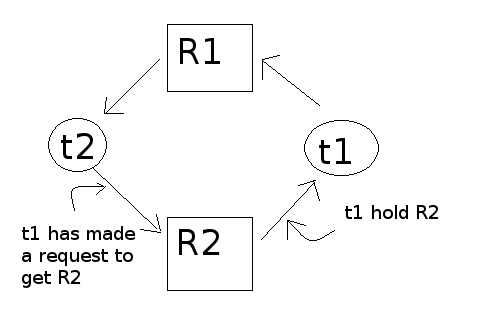
\includegraphics[scale =0.6]{resource_allocation_graph.png}
    \caption{Resource allocation graph}
  \end{center}
\end{figure}

There is a circular wait in the system if there is a cycle in this graph.
$=>$ Detecting a deadlock is easy using this graph ( using, for instance, a bellman-ford algorithm).

Another way to use this graph is to perform a cycle detection for each new request and to decide to refuse it if this induces a cycle in the graph.
This model is not suited if resources are divided into types and if threads ask for one instance of a given resource.
It can be extended :

\begin{figure}[h]
  \begin{center}
    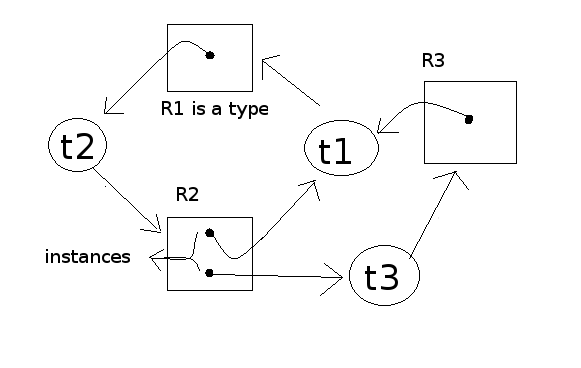
\includegraphics[scale=0.6]{resource_graph_extended}
    \caption{Extended resource allocation graph}
  \end{center}
\end{figure}

In this model, the presence of a cycle doesn't necessarily means that there is a deadlock, only a set of cycles that saturates all the resources it contains, will be a deadlock. $-->$ Not practical.

\section{Allocation matrices and banker algorithm}

\subsection{Hypothesis}

At first we assume that we know :

\begin{itemize}
  \item a vector Available such that : Available[i] = number of instances of resources i that are available.
  \item a matrix Allocation such that : Allocation[i][j] = number of resources of type i allocated to thread j.
  \item a matrix Max such that : Max[i][j] = maximal number of resources of type i the thread j will need.
  \item a matrix Need such that : Nedd[i][j] = Max[i][j] - Allocation[i][j]
\end{itemize}

We will try to find if there is an order that make the execution of all threads possible :

\begin{enumerate}
  \item Work = Available
  \item Finished[j] = false for all threads.
  \item while there is some thread j such that : \\ Finished[j] = false \&\& Noeud[i][j] $\leq$ Work[i] $\forall$, \\then : Work[i] += Allocation[i][j] $\forall$ i ; \\Finished[j] =true;
  \item if there is a j such that Finished[j] = false, the system is not in a safe state.
\end{enumerate}

This previous algorithm finds out if the system is in a safe state or not.

For deadlock prevention, we use the banker algorithm : when an allocation request is issue to the system :

\begin{enumerate}

  \item Pretend the request is granted : \\ Available -= request; \\ Allocation[*][j] += request;
  \item run the safe state detection
  \item if the state is not safe, rollback and deny the request.
  
\end{enumerate}

\subsection{Example of the banker algorithm}


  \begin{center}
  Threads
    \begin{tabular}{ccccccc}
       Allocation& A B C & &Available & & Need & A B C\\
       0 & 1 0 1 & & (\textbf{0})1 0 2 & & 0 & 0 2 0 \\
       1 & 0 0 1 & &  & & 1 & 2 1 0\\
       2 & 0 2 0 & &  & & 2 & 0 0 1\\
       3 & (\textbf{2})1 0 0 & &  & & 3 & (\textbf{1})2 2 0\\
       4 & 2 0 0 & &  & & 4 & 2 2 3\\
    \end{tabular}
  \end{center}

Assume that thread 3 requests 1 A resource (1,0,0) (represented in the example with the new numbers between paranthesis)
\begin{enumerate}
  \item Pretend the request is accepted
  \item Run the algorithm to know if the state is safe : Work = (0,0,2). 

  \begin{center}
    \begin{tabular}{cc}
      Thread & Finished\\
      0 & f\\
      1 & f\\
      2 & f\\
      3 & f\\
      4 & f\\
    \end{tabular}
  \end{center}

Thread 2 has needs $\leq$ Work  : Work = (0,2,2).

Thread 0 has needs $\leq$ Work : Work = (1,2,3).

Thread 3 has needs $\leq$ Work : Work = (3,2,3).

Thread 4 has needs $\leq$ Work : Work = (5,2,3).

Thread 1 has needs $\leq$ Work : Work = (5,2,4).

So now we get :

\begin{center}
    \begin{tabular}{cc}
      Thread & Finished\\
      0 & t\\
      1 & t\\
      2 & t\\
      3 & t\\
      4 & t\\
    \end{tabular}
  \end{center}

\item Finished is filled with "true" $=>$ the request can be granted.
\end{enumerate}

Assume that thread 4 requests 1A resource and 1C resource (1,0,1).

\begin{enumerate}
  \item if the request is $>$ Need(thread), or $>$ Available, deny it.
  \item Pretend the request is accepted.
  \item run the algorithm to know if the state is safe : Work =(0,0,1)
  
Thread 2 has needs $\leq$ Work  : Work = (0,2,1).

Thread 0 has needs $\leq$ Work : Work = (1,2,2).

Thread 3 has needs $\leq$ Work : Work = (4,2,3).

Thread 4 has needs $\leq$ Work : Work = (5,2,3).

Thread 1 has needs $\leq$ Work : Work = (5,2,4).

So now we get again :

\begin{center}
    \begin{tabular}{cc}
      Thread & Finished\\
      0 & t\\
      1 & t\\
      2 & t\\
      3 & t\\
      4 & t\\
    \end{tabular}
  \end{center}
  
  \item the request is granted
\end{enumerate}

Running time of the safe state algorithm is $n^2*m$ where n is the number of threads and m the number of resource types $=>$ Costly, repeated for each allocation request.


Global method : you compare the available vector with the needs vectors.
If there is any need vector which is lower than available, the threads order will start with this one, and will release his allocated resources.
Therefore, Thread order += Thread X and Available += Allocation of X
Then, you repeat until all threads are ordered or when you are stuck.
All states will be safe or one won't be.

\section{Detecting Deadlocks vs Preventing them}

Let run the system without doing anything and look for a deadlock periodically.
Using the resource allocation graph, it's the same algorithm to prevent or detect : find a cycle in the graph.
using Allocation matrix : we take an optimistic approach, we assume that thread don't need any more resources $=>$ we replace the "Need" Matrix with pending requests, then use the safe state detection to find out if there is a deadlock

If a deadlock is detected :
\begin{itemize}
  \item preempt resources $->$ not always possible.
  \item kill some of the threads :
  \begin{itemize}
    \item the minimal number of threads that restores a safe state ?

$=>$ risk of killing important threads ( ex : Window manager, command interpreter...)
    \item killing threads that are not related to the system.
    \item let the user decide.
    \item choose at random...
  \end{itemize}
\end{itemize}

In most systems, deadlocks are not handled at all.
One canf find them in :
\begin{itemize}
  \item some experimental OS
  \item some debugging environments
\end{itemize}



\end{document}

\documentclass[a4paper,10pt]{article}

%%%% PRATIQUE POUR LES ALINEAS CHIANTS
\usepackage{indentfirst}

%%%% POUR L'OPTION LABEL= %%%
\usepackage{enumitem}

\setlength{\parindent}{30pt}
\setlength{\parskip}{1ex}
\setlength{\textwidth}{15cm}
\setlength{\textheight}{24cm}
\setlength{\oddsidemargin}{0.2cm}
\setlength{\evensidemargin}{-.7cm}
\setlength{\topmargin}{-.5in}

\usepackage{graphicx}
\usepackage{titling}
\usepackage{listings}
\lstset{%
  basicstyle=\scriptsize\sffamily,%
  commentstyle=\footnotesize\ttfamily,%
  frameround=trBL,
  frame=single,
  breaklines=true,
  showstringspaces=false,
  numbers=left,
  numberstyle=\tiny,
  numbersep=10pt,
  keywordstyle=\bf
}
\newcommand{\subtitle}[1]{%
  \posttitle{%
    \par\end{center}
    \begin{center}\large#1\end{center}
    \vskip0.5em}%
}
\title{\textbf{Synchronization}}
\subtitle{M1 MoSIG : Operating Systems}
\author{Poupin Pierre \and Rouby Thomas}
\date{04/11/2014}

\begin{document}
\maketitle
%\begin{abstract}
%This document is our report of the first practical session. It contains our design choices along with the results of our implementation.	
%\end{abstract}



\section{Semaphores}

Proposed by Dijkstra, Semaphores are special counters on which 2 operations are defined :
\begin{itemize}
  \item P or wait on a semaphore s :
    \begin{verbatim}
      if (s.counter == 0)
        wait
        s.counter--
    \end{verbatim}
  \item V or post on a semaphore s :
  \begin{verbatim}
      s.counter++
  \end{verbatim}
\end{itemize}

\subsection{Typical use :} 

\begin{itemize}
  
\item restrict the access to a region to a fixed number of threads.
Example :

\begin{verbatim}
    s = semaphore initialized to N
    threads execute :
        wait(s);
            restricted section;
        post(s);
\end{verbatim}

\item as a lock (binary semaphore).
Example :
\begin{verbatim}
  s = semaphore initialized to 1
  Some code as above for threads.
\end{verbatim}
\end{itemize}

\subsection{Example: Procuder/Consumer}

\begin{figure}
  \begin{center}
    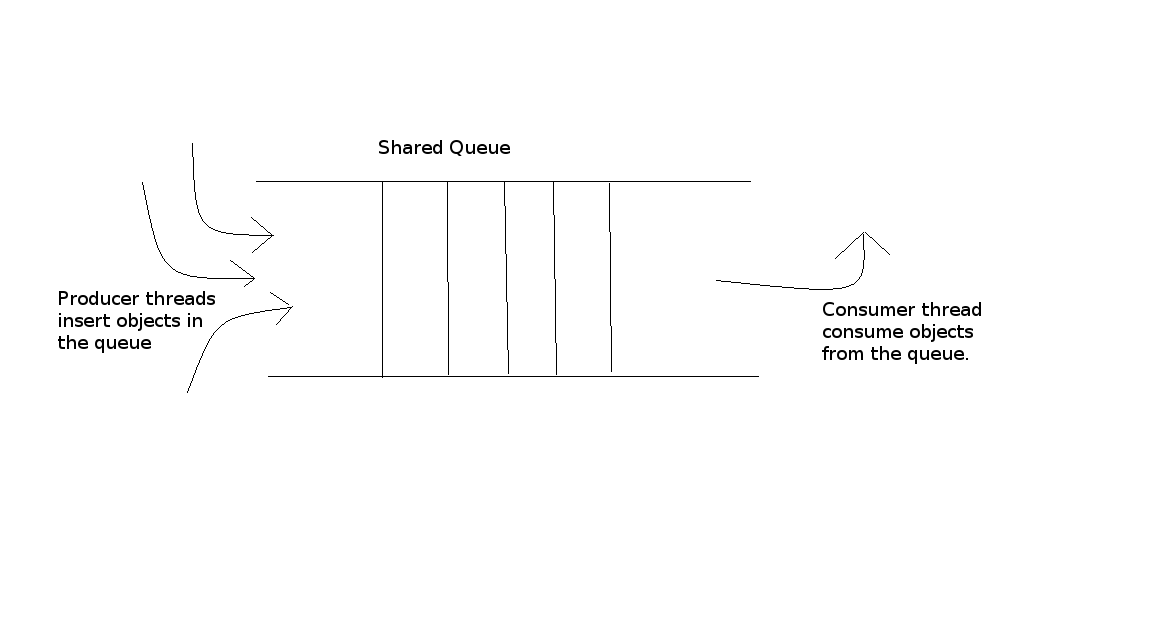
\includegraphics[scale=0.5]{shared_queue.png}
    \caption{Situation of the producer/consumer example}
    \label{}
  \end{center}
\end{figure}

In this example, we will use a circular buffer of size N as our queue.
If an operation is not possible, threads wait until the operation is possible.
\begin{verbatim}
semaphore s = 1, available = N, occupied = 0;

produce(int object) {

     //possibility to wait
     wait(available);
     // at most N producers
     wait(s);
     queue.buffer[(queue.head + queue.size) % N ] = object;
     queue.size++;
     post(s);
     post(occupied);
}

int consume() {
     int result;
     wait(occupied);
     // number of consumers waiting bounded...
     wait(s);
     result = queue.buffer[queue.head];
     queue.head = (queue.head +1) % N;
     queue.size--;
     post(available);
     post(s);
}
//Idea : use semaphores to count :
// the number of available slots (semaphore initialized to N)
// the number of occupied slots (semaphore initialized to 0)

Comment on the code: complicated because the order of wait operation matters.
\end{verbatim}



\subsection{Implementation of Semaphores :}

A semaphore is :
\begin{itemize}
  \item an integer value : counter
  \item a list of blocked processes : l
  \item a boolean variable : lock
\end{itemize}
\begin{verbatim}
  typedef struct{
  int lock;
  list l;
  int counter;
  } semaphore_t;
  
  // initially, lock=0, l is empty, counter is defined at semaphore creation
  
  void wait(semaphore_t s){
       while(test_and_set(&s.lock,1) {}
       if (s.counter>0){
            s.counter--;
            s.lock =0;
       }
       else{
            tid = get_current_thread_id();
            unschedule(tid);
            mark_as_blocked(tid);
            insert(s.l,tid);
            s.lock = 0;
            schedule();
       }
  }
  
  void post(semaphore_t s) {
       while(test_and_set(&s.lock,1) {}
       if (is_empty(s.l)){
            s.counter++;
            s.lock =0;   
       }
       else {
            tid = remove(s.l);
            mark_as_unblocked(tid);
            s.lock = 0;
       }
  }
  
  Comment : the wait operation takes advantage of the scheduler to perform its task.
\end{verbatim}

\section{Monitors}

Introduced by Haare, monitors are objects in which methods are executed in mutual exclusion.

\begin{tabular}{cccc}
  threads & \vdots & \vdots & \vdots
\end{tabular}
|
| 
\textgreater
\begin{tabular}{|c|}
 attributes \\
 : \\
 : \\
 : \\
\end{tabular}

Only one thread at a time can execute something inside the monitor .

This model makes things simpler because it is not necessary to manage locks anymore.

\subsection{Example: Producer/Consumer}

The queue will be implemented as a monitor, with buffer, size, head as attributes and two methods :

Thr monitors support two operations :
\begin{itemize}
  \item wait(condition C) : releases the access to the monitor then waits until some signal is sent on C, then compete for the lock to retrieve access to the monitor.
  \item signal(condition C) : sends a signal on C. The signal is lost if no thread waits on C.
\end{itemize}
 
 
 \begin{verbatim}
 
  condition not_full , not_empty;
  
   produce(int object){
        while(size==N)
        wait(not_full);
        buffer[(head+size)%N] =object;
        size++;
        signal(not_empty);
   }
   
   int consume(){
        int result;
        while(size==0)
        wait(not_empty);
        result = buffer[head];
        head =(head+1)%N;
        size--;
        signal(not_full);
   }
 \end{verbatim}


\subsection{Implementation}

Similar to semaphores. Notice that both models are equivalent. It is possible to implement one of them using the other.
\end{document}

\documentclass[a4paper,10pt]{article}

%%%% PRATIQUE POUR LES ALINEAS CHIANTS
\usepackage{indentfirst}

%%%% POUR L'OPTION LABEL= %%%
\usepackage{enumitem}

\setlength{\parindent}{30pt}
\setlength{\parskip}{1ex}
\setlength{\textwidth}{15cm}
\setlength{\textheight}{24cm}
\setlength{\oddsidemargin}{0.2cm}
\setlength{\evensidemargin}{-.7cm}
\setlength{\topmargin}{-.5in}

\usepackage{graphicx}
\usepackage{titling}
\usepackage{listings}
\lstset{%
  basicstyle=\scriptsize\sffamily,%
  commentstyle=\footnotesize\ttfamily,%
  frameround=trBL,
  frame=single,
  breaklines=true,
  showstringspaces=false,
  numbers=left,
  numberstyle=\tiny,
  numbersep=10pt,
  keywordstyle=\bf
}
\newcommand{\subtitle}[1]{%
  \posttitle{%
    \par\end{center}
    \begin{center}\large#1\end{center}
    \vskip0.5em}%
}
\title{\textbf{Synchronization without locks}}
\subtitle{M1 MoSIG : Operating Systems}
\author{Poupin Pierre \and Rouby Thomas}
\date{18/11/2014}

\begin{document}
\maketitle
%\begin{abstract}
%This document is our report of the first practical session. It contains our design choices along with the results of our implementation.	
%\end{abstract}


Synchronization primitives are costly :
\begin{itemize}
  \item spinlocks :
  \begin{itemize}
    \item atomic instruction that locks the memory bus
    \item active wait
  \end{itemize}
  \item semaphore/monitor :
  \begin{itemize}
    \item risk of being unscheduled : cost of switch
    \item entering in the kernel
  \end{itemize}
\end{itemize}

Notice that actual implementation of locks in system such as Linux is a mix between spinlock and unscheduling of the thread.

Other solutions :

\begin{itemize}
  \item algorithmic changes : no more critical sections
  
  Example : Producer/Consumer
  
  \begin{center}
size\\buffer\\head

      \begin{tabular}{c|c}
        Producer & Consumer\\
        while(size==N) {} & while(size==0) {}\\
        buffer[(head+size)\%N]= object & result = buffer[head]\\
         & head=(head+1)\%N \\        
        size++ & size -- \\
      \end{tabular}
    \end{center}
  
  
  \begin{itemize}
    \item forget about size
    \item use head and tail
    \item single producer/consumer
    \item SC
  \end{itemize}

So we get :
\begin{center}
tail\\buffer\\head

      \begin{tabular}{c|c}
        Producer & Consumer\\
        while((tail+1)\%N==head) {} & while(head==tail) {}\\
        buffer[tail]= object & result = buffer[head]\\
        tail = (tail+1)\%N & head=(head+1)\%N \\        
      \end{tabular}
    \end{center}    

\item take advantage of atomic instructions

Example : 
\begin{verbatim}

Compare_and_Swap(address,old,new)
 if(*address ==old) {
    *address=new;
    return 1;
 }
 else return 0;
\end{verbatim}
can be used to write an atomic stack :

\begin{verbatim}
  void atomic_push(stack* s, int value) {
      item = malloc(sizeof(node));
      item->val = value;
      do {
          item->next = *s;
      } while (compare_and_swap(s, item->next, item);
  }
\end{verbatim}

Similar for atomic\_pop (try to set s to *s-$>$next atomically)

\end{itemize}

Other performance issues include :

\begin{itemize}
  \item locks locality: with non uniform memories or with non uniform caches. $=>$ more elaborate locking structures (hierarchical, or distributed and made coherent)
  \item bottlenecks: if a single lock is used by all the threads $=>$ it's better to separate the work into independant parts and use several locks.
\end{itemize}

\end{document}

\documentclass[a4paper,10pt]{article}

%%%% PRATIQUE POUR LES ALINEAS CHIANTS
\usepackage{indentfirst}

%%%% POUR L'OPTION LABEL= %%%
\usepackage{enumitem}

\setlength{\parindent}{30pt}
\setlength{\parskip}{1ex}
\setlength{\textwidth}{15cm}
\setlength{\textheight}{24cm}
\setlength{\oddsidemargin}{0.2cm}
\setlength{\evensidemargin}{-.7cm}
\setlength{\topmargin}{-.5in}

\usepackage{graphicx}
\usepackage{titling}
\usepackage{listings}
\lstset{%
  basicstyle=\scriptsize\sffamily,%
  commentstyle=\footnotesize\ttfamily,%
  frameround=trBL,
  frame=single,
  breaklines=true,
  showstringspaces=false,
  numbers=left,
  numberstyle=\tiny,
  numbersep=10pt,
  keywordstyle=\bf
}
\newcommand{\subtitle}[1]{%
  \posttitle{%
    \par\end{center}
    \begin{center}\large#1\end{center}
    \vskip0.5em}%
}
\title{\textbf{Low level inputs/outputs}}
\subtitle{M1 MoSIG : Operating Systems}
\author{Poupin Pierre \and Rouby Thomas}
\date{18/11/2014}

\begin{document}
\maketitle

\section{Introduction}

Architecture of a typical device :

\begin{figure}[h!]
  \begin{center}
    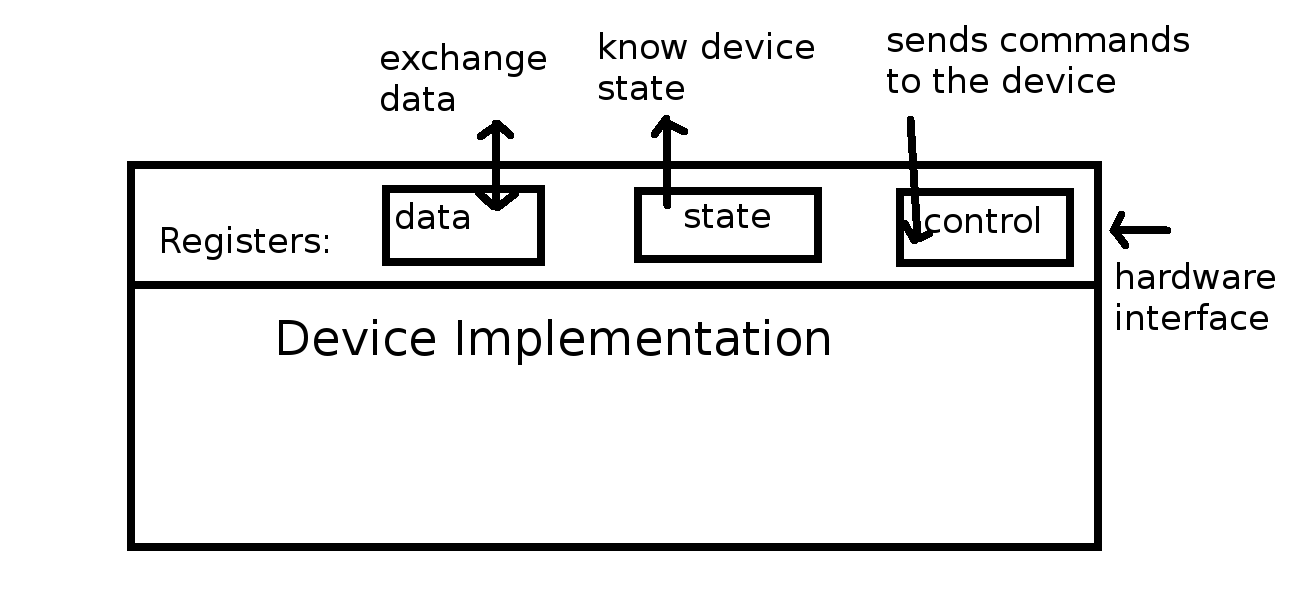
\includegraphics[width=0.8\textwidth]{architecture_device.png}
    \label{Architecture of a typical device}
  \end{center}
\end{figure}
This general scheme applies to : hard drives, printers, mouses...


Computer layout :
\begin{figure}[h!]
  \begin{center}
    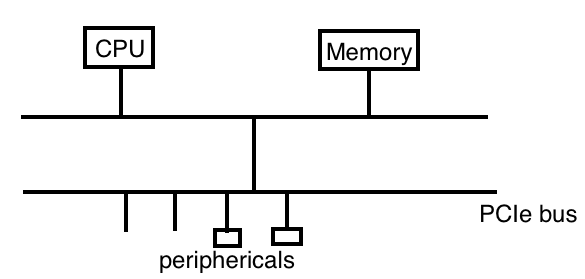
\includegraphics[width=0.8\textwidth]{computer_layout.png}
    \label{fig:1}
  \end{center}
\end{figure}

To access to periphericals, one has to issue either :

\begin{itemize}
  \item special instructions to write to one of the I/O registers of periphericals.
  A port is provided which is the target device.
  
  \item memory access ... . The address space is divided into :
  \begin{itemize}
    \item  main memory
    \item 16 registers of periphericals
  \end{itemize}
\end{itemize}

Basic exchange with a peripherical :

\begin{verbatim}
  while(read(status) == busy) 
  {}
  write(data,some_data);
  write(control,some_command);
  while(read(status)==busy) 
  {}
\end{verbatim}



\section{Device Driver}

The OS would rather handle generic periphericals: for instance, a storage device should look like a sequence of data block

\begin{table}[h]
\begin{tabular}{llllllll}
0                      & 1                     & 2                     & 3                     & 4                     & 5                     & 6                     & 7                     \\ \hline
\multicolumn{1}{|l|}{} & \multicolumn{1}{l|}{} & \multicolumn{1}{l|}{} & \multicolumn{1}{l|}{} & \multicolumn{1}{l|}{} & \multicolumn{1}{l|}{} & \multicolumn{1}{l|}{} & \multicolumn{1}{l|}{} \\ \hline
\end{tabular}
\end{table}
%place table here

Along with two properties :
\begin{itemize}
  \item read(int num\_block, void *result);
  \item write(int num\_block, void *result);
\end{itemize}

A driver is a piece of the OS that provides that kind of abstraction for a specific device type.

\textbf{Example:}

An IDE driver, writing to the disk looks like :
\begin{itemize}
  \item loop waiting for disk availability.
  \item write the block number (28 bits) and the drive number into 4 controls registers.
  \item wait for device availability for data transfer
  \item transfer the data :
  \begin{itemize}
    \item write a data piece (usually 4 bytes) to the data register
    \item write a signal to the command register
    \item wait for completion (polling the status register)
  \end{itemize}
  Repeat until all the data is transfered.
  \item wait for the completion of the operation
  \item report a possible error
\end{itemize}

\begin{figure}[h!]
  \begin{center}
    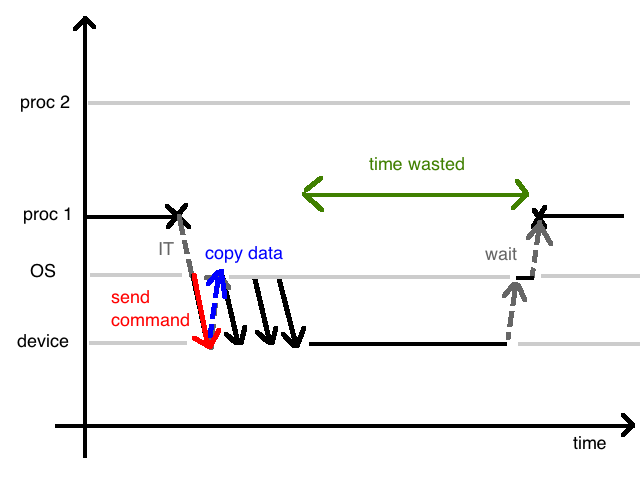
\includegraphics[width=0.8\textwidth]{resources_wasted.png}
    \label{fig:2}
  \end{center}
\end{figure}

\section{Improving resources utilization}
Devices are usually much slower than CPU, We can improve resources utilization, by avoiding active wait.

\subsection{Poll on a regular basis}

\begin{figure}[h!]
  \begin{center}
    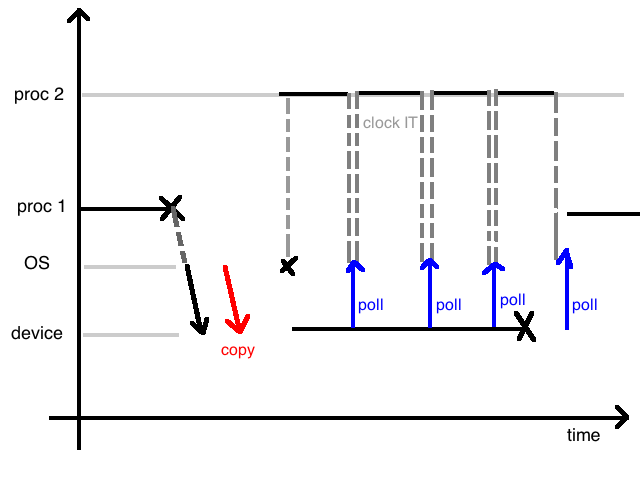
\includegraphics[width=0.8\textwidth]{poll.png}
    \label{fig:3}
  \end{center}
\end{figure}

Issues :

\begin{itemize}
  \item Several polls to the device
  \item The device is not used between the completion of the request and the next poll.
\end{itemize}

\subsection{Use Interrupts}

Now the device has the capacity to raise an interrupt (typically at request completion).

\begin{figure}[h!]
  \begin{center}
    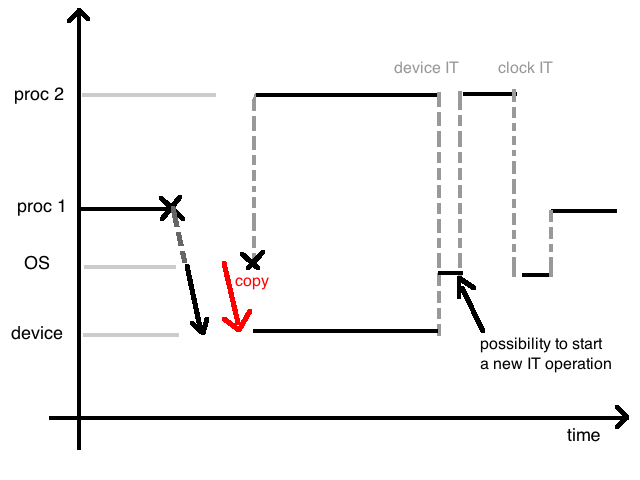
\includegraphics[width=0.8\textwidth]{interrupt.png}
    \label{fig:4}
  \end{center}
\end{figure}

Issues : The CPU is not used efficiently during the copy.

\subsection{Use DMA}

\begin{figure}[h!]
  \begin{center}
    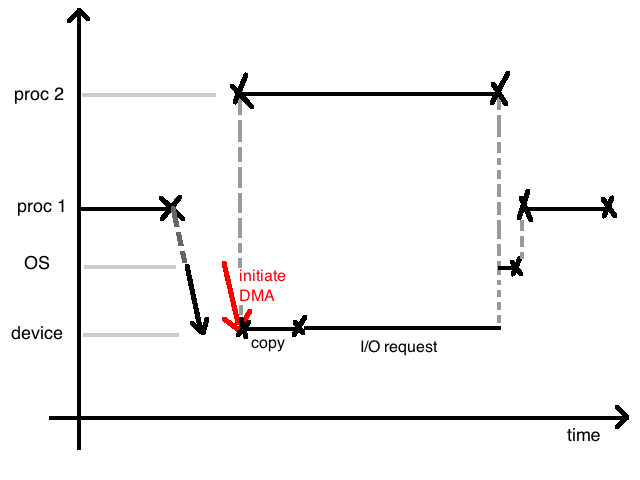
\includegraphics[width=0.65\textwidth]{dma.png}
    \caption{DMA}
    \label{fig:5}
  \end{center}
\end{figure}

DMA stands for Direct Memory Access, it has to be handled both by :
\begin{itemize}
  \item the memory controller
  \item the device
\end{itemize}

It let a device exchange data blocks with the memory without the need of the CPU.
The CPU just has to initiate the access.


DMA is used for fast devices :
\begin{itemize}
  \item hard disks
  \item CD Roms
  \item graphic accelerator
\end{itemize}

\section{Up to the user interface}

\begin{figure}[h!]
  \begin{center}
    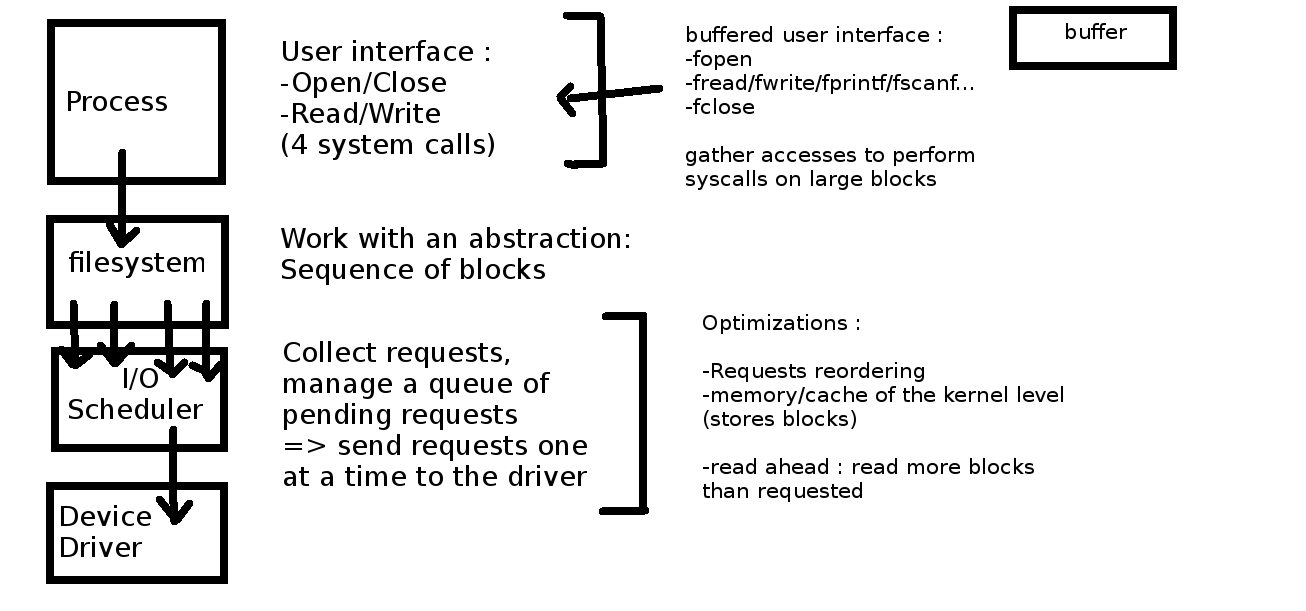
\includegraphics[width=\textwidth]{user_interface.png}
    \label{fig:6}
  \end{center}
\end{figure}

\end{document}

\chapter{Input/Output scheduling}
\section{Introduction, hard drives technology}

Algorithms for I/Os scheduling in use today are motivated by mechanical hard drives technology.
A mechanical hard drive is made :
\begin{itemize}
  \item platters (rotating) on which data is stored.
  \item arm to move r/w heads.
  \item r/w head at the end of the arm.
\end{itemize}

\begin{figure}[h!]
  \begin{center}
    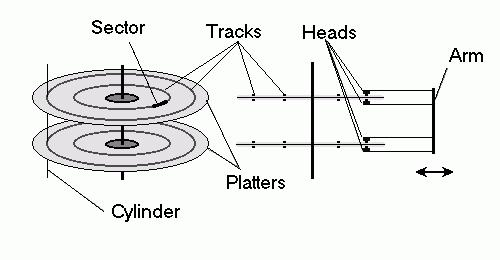
\includegraphics{hard_drive_picture.jpg}
  \end{center}
\end{figure}

%place hard drive picture here
To perform an access to a specific sector :
\begin{itemize}
  \item move the arm to the proper track
  $=>$ takes time: depends on the engine moving the arm.
  \item wait for the desired sector
   $=>$ takes time: depends on the rotating speed of the platters.
  \item select the head and read or write
  $=>$ fast.
\end{itemize}

As a result, the access time to some sector will be :
\begin{itemize}
  \item fast: if the arm is already on the right track and the sector already under the r/w head. (about 125 MB/s $=>$ 500 nanoseconds to get 4 bytes).
  It is the bandwidth of sequential accesses.
  \item slow: otherwise (about 10 ms to get 4 bytes : there is a 20 000 factor).
  It is the latency of a random access.
  
\end{itemize}

Usually, sequential accesses can reach full bandwidth with a small degradation on track change.
Latency is given on average, the exact latency depends on the istance of the arm from the track and on the sector position.

\section{I/Os scheduling}

The CPU is much faster than a hard disk, even at full bandwidth, there is a possibility to produce more I/O requests than the drive can handle

$=>$ queue of pending requests in the kernel

$=>$ optimizations: reordering, aggregation.

\subsection{FcFs (First come First served)}

\begin{figure}[h!]
  \begin{center}
    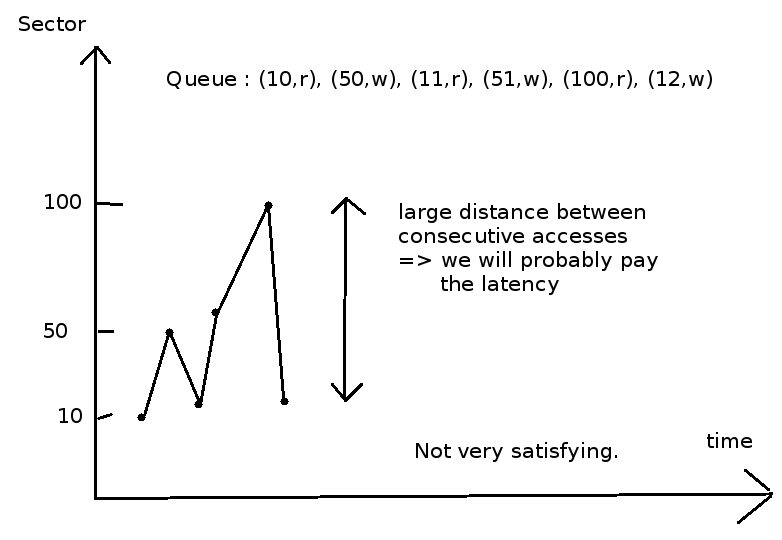
\includegraphics[width=0.6\textwidth]{fcfs.png}
  \end{center}
\end{figure}

\subsection{SSTF ( SSF, NBF)}

Shortest seek-time first of shorter seek first or nearest block first.

\begin{figure}[th!]
  \begin{center}
    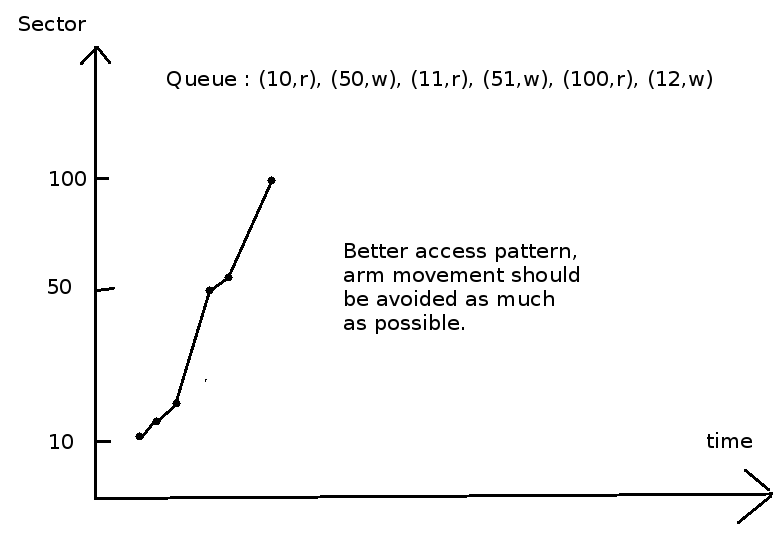
\includegraphics[width=0.6\textwidth]{sstf.png}
  \end{center}
\end{figure}

But :

\begin{itemize}
  \item adjacent accesses are the best if they are on the same track
  
  $=>$ should be improved by taking into account :
  
  
  (The geometry of the drive is not given to the OS). 
  \begin{itemize}
    \item number of tracks to cross
    \item time to wait for the sector once on the right track
  \end{itemize}
 
  
  $=>$ might be implemented in the disk itself (SCSI and SATA)
  
  \item starvation: if requests close the current head position arrive constantly.
  This is especially true for requests close to the ends of the disk.
\end{itemize}

\subsection{SCAN/LOOK/the elevator}

This algorithm serve requests in two phases :

\begin{itemize}
  \item first by increasing order of sector number
  \item secondly by decreasing order of sector number
\end{itemize}
Then it loops over these two phases.

\begin{figure}[h!]
  \begin{center}
    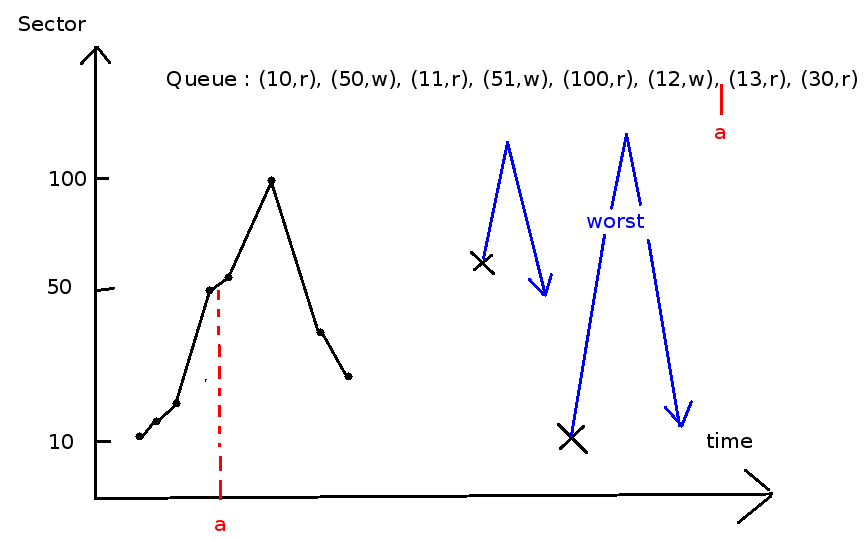
\includegraphics[width=0.8\textwidth]{elevator.png}
    \label{fig:1}
  \end{center}
\end{figure}

Advantages :

\begin{itemize}
  \item Some locality, close requests already in the queue will be grouped
  \item no starvation, the head moves strictly toward the last request in one direction.
\end{itemize}

Drawbacks :

\begin{itemize}
  \item accesses in the wrong direction are not necessarily efficient in the disk.
  \item requests on the middle of the disk have a better serving time $=>$ fairness issue
\end{itemize}

\subsection{Circular SCAN}

Serve request only by increasing sector number. Rewind to the request nearest to the beginning of the disk when the request with the largest sector number is served.
\begin{figure}[h!]
  \begin{center}
    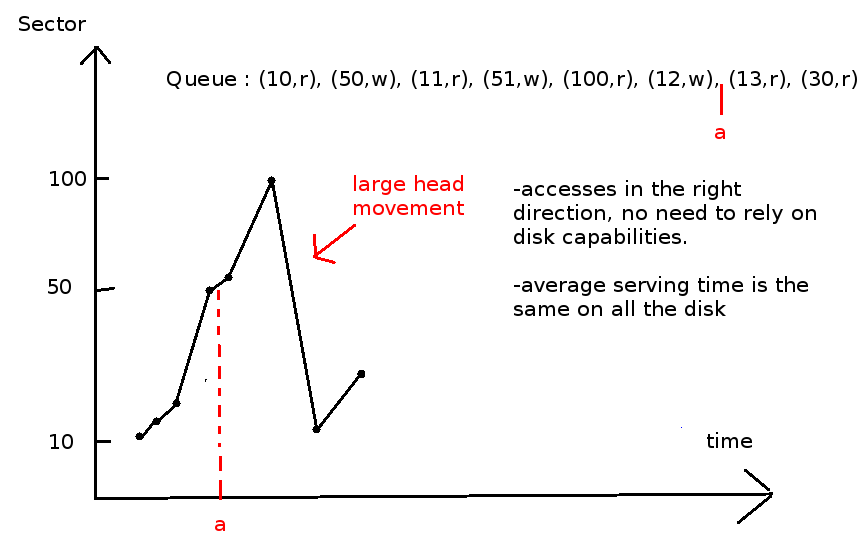
\includegraphics[width=0.8\textwidth]{circular.png}
    \caption{Circular Scan}
    \label{fig:2}
  \end{center}
\end{figure}
\subsection{Anticipatory scheduling}

Do not apply the work-first principle; when a process is performing a sequential access, all the requests are not necessarily in the queue.

The idea is to wait a little time after a request to let the opportunity to the served process to issue the next request

\subsection{Other strategies}
\begin{itemize}
  \item Deadline scheduling :
  requests are served by optimizing locality (SSTF with anticipatory waits) but are also associated with a deadline after which they will be served in priority.
  
  $=>$ no starvation
  
  \item fair queuing :
  each process has its own queue, the scheduler divied "fairly" the time during which a process can have its requests served.
\end{itemize}

\section{Conclusion}

These algorithms assume that :
\begin{itemize}
  \item sequential accesses are much faster than random ones (because of the 20 000 factor)
  \item it is worth spending time reordering requests ( very large gain).
  \item seek time depends on the distance between sectors.
\end{itemize}

But it is not completely true with newer technologies (SSD).



\end{document}
